
%%% PAGE DIMENSIONS
%\usepackage{geometry} % to change the page dimensions
%\geometry{a4paper} % or letterpaper (US) or a5paper or....
%\geometry{margin=2in} % for example, change the margins to 2 inches all round
%\geometry{landscape} % set up the page for landscape

%%% PACKAGES
%\usepackage{graphicx} % support the \includegraphics command and options
%\usepackage[parfill]{parskip} % Activate to begin paragraphs with an empty line rather than an indent
%\usepackage{amsmath, amsfonts}
%\usepackage{booktabs} % for much better looking tables
%\usepackage{array} % for better arrays (eg matrices) in maths
%\usepackage{paralist} % very flexible & customisable lists (eg. enumerate/itemize, etc.)
%\usepackage{verbatim} % adds environment for commenting out blocks of text & for better verbatim
%\usepackage{subfig} % make it possible to include more than one captioned figure/table in a single float
%These packages are all incorporated in the memoir class to one degree or another...


\iffalse

%%% SECTION TITLE APPEARANCE
\usepackage{sectsty}
\allsectionsfont{\sffamily\mdseries\upshape}

\newcommand{\N}{\mathbb{N}}
\newcommand{\Z}{\mathbb{Z}}
\newcommand{\R}{\mathbb{R}}
\newcommand{\Q}{\mathbb{Q}}

\fi

%%% The "real" document content comes below...


\documentclass[12pt,fleqn]{article}
\usepackage{latexsym,epsf,amssymb,amsmath}
\usepackage{geometry}
\usepackage{graphicx}
\geometry{margin=1in}

\def\Homework{6}%Number of Homework
\def\Session{Spring 2015}
\def\Name{Nguyet Duong} % Fill in your name here

\markboth{}{CS70, \Session, HW \Homework, \Name}
\pagestyle{myheadings}

\title{CS 70, \Session\ --- Solutions to Homework \Homework}
\date{}

\begin{document}
\maketitle

\section*{Due Monday March 2 at 12 noon}


%%% EVERYTHING BELOW THIS WILL REMAIN THE SAME!!!

\begin{enumerate}
  
  \item \textbf{RSA lite} 
  
  We are given $e = 67$, $P = 101$. We also know $35 = m^{e}$ (mod P). 
  From the RSA algorithm, we know that the equation can be considered like $E(m) = m^{e}$ (mod P), where $E(m) = 35$ in this case. That means we can use the following to find what m is: $m = E(m)^{d}$ (mod P). 
  
  We can do this from Theorem 7.2 which states $E(m)^{d} = m$ (mod P), which is essentially $(m^{e})^{d} = m$ (mod P). So now we need to find a d in order to solve for m. 
  
  d must be the multiplicative inverse of e (mod P). This means: $ed = 1$ (mod P). We can find this through Euclid's Algorithm. 
  \begin{align*} 
	67d &= 1 \:(mod\: 101) \\
	101 &= 67(1) + 34 \\
	67 &= 34(1) + 33 \\
	34 &= 33(1) + 1 
  \end{align*}
  Note that: 
  \begin{align*} 
	33 &= 67 + (-1)34 \\
	34 &= 101 + (-1)67 
  \end{align*} 
  Now we can do the following:
  \begin{align*} 
	1 &= 34 + (-1)33 \\
	1 &= 34 + (-1)(67 + (-1)34)\\
	1 &= 34 + (-1)67 + 34\\
	1 &= (2)34 + (-1)67\\
	1 &= 2(101 + (-1)67) + (-1)67\\
	1 &= 2(101) + (-2)67 + (-1)67 \\
	1 &= 2(101) + (-3)67\\
  \end{align*} 
  This means that we can find our number by doing $101 - 3 = 98$. So $d = 98$. Knowing this, we can finally plug into our equation $35^d = m$ (mod P). Which is equivalent to $35^{98} = m$ (mod P). We can find out what m is by evaluating the left hand side in the following manner:
  
  \begin{itemize}
  	\item Notice that 98 in binary is 0110 0010. We have 1's in the following positions: 2, 32, and 64. These add up to become 98. 
  	\item That means we can do the following using algebra: $35^{98} = 35^{2} * 35^{32} * 35^{64}$. We can find the mod of each individually and multiply it together then take the mod of that.
  	\begin{align*} 
	35^{2} &= 13 \: (mod \: 101) \\
	35^{4} &= (35^{2})^{2} = 13^2 = 68 \: (mod \: 101) \\
	35^{8} &= (35^{4})^{2} = 68^2 = 79 \: (mod \: 101) \\
	35^{16} &= (35^{8})^{2} = 79^2 = 80 \: (mod \: 101) \\
	35^{32} &= (35^{16})^{2} = 80^2 = 37 \: (mod \: 101) \\
	35^{64} &= (35^{32})^{2} = 37^2 = 56 \: (mod \: 101) 
  \end{align*} 
  \item So plugging it back into the equation we had above, we get the following: $13 * 37 * 56 = 70$ (mod 101).
  \item Hence our message $m = 70$. 
  \end{itemize}
  
  \newpage
  \item \textbf{Fermat and CRT}

  \begin{enumerate}
    \item 
    Some key points we need to note is that P and Q are odd primes, and as a result, their $gcd(P,Q) = 1$. Knowing this, we can use the Chinese Remainder Theorem (CRT) in order to prove that $x^{(P - 1)(Q - 1)} \equiv y \: (mod \: N)$ when $N = PQ$. So using the CRT, we can make our LHS be the unique C (mod N). This that there are $r_1$ and $r_2$ such that $x^{(P - 1)(Q - 1)} \equiv r_1 \: (mod \: P)$ and $x^{(P - 1)(Q - 1)} \equiv r_2 \: (mod \: Q)$. From our given, we know that $r_1 = r_2 = y$.
    
    Now using the modulo arithmetic, we know the following: 
    
    \begin{itemize}
    		\item $x^{(P - 1)(Q - 1)}  \equiv y$ (mod P), and $N \mid P$ (from our given), then we can say $x^{(P - 1)(Q - 1)}  \equiv y$ (mod N)
    		\item $x^{(P - 1)(Q - 1)}  \equiv y$ (mod Q), and $N \mid Q$ (from our given), then we can say $x^{(P - 1)(Q - 1)}  \equiv y$ (mod N)
    \end{itemize}
    
    Hence we can say that $x^{(P - 1)(Q - 1)} \equiv y \: (mod \: N)$.
    
    \item 
	Using modulo arithmetic, we can do the following:
	\begin{align*}
		&x^{(P - 1)(Q - 1)} = x^{P-1} * x^{Q-1} \\
		&a = x^{P-1} \\
		&b = x^{Q-1} \\
		&a \equiv 1 \: (mod \: P) \: by \: Fermat's \: Little \: Theorem \\ 
		&let \: b \equiv d_1 \: (mod \: P) \\
		&Using \:modulo \:arithmetic, \:we \:can \:do \:the \: following: \\ 
		&a * b = 1 * d_1 \: (mod \: P) \\
		&Therefore , \: x^{(P - 1)(Q - 1)} \equiv d_1 \: (mod \: P) \\
		&b \equiv 1 \: (mod \: Q) \: by \: Fermat's \: Little \: Theorem \\ 
		&let \: a \equiv d_2 \: (mod \: Q) \\
		&Using \:modulo \:arithmetic, \:we \:can \:do \:the \: following: \\ 
		&a * b = 1 * d_2 \: (mod \: Q) \\
		&Therefore , \: x^{(P - 1)(Q - 1)} \equiv d_2 \: (mod \: Q) 
	\end{align*}
    Now we make an observation that $d_1 = d_2 = y$ because from what we were given above. Since one of the multiples was 1, it has to be the same value in order to get the value given to us (y). 
    \item 
    Using the CRT and what we reasoned out in the above, we will end up doing the following:
    
    $x^{(P - 1)(Q - 1)} \equiv d_1$ (mod P). Note that what needs to be evaluated/find ($d_1$) the remainder in this situation is actually $x^{Q-1}$. Similarly the other way around, $x^{(P - 1)(Q - 1)} \equiv d_2$ (mod Q) with $d_2$ to be the remainder of the situation to be $x^(P-1)$. So when we apply the CRT, we have both P and Q so that we can apply Fermat's Little Theorem to the $x^{P -1}$ and $x^{Q-1}$ so that both of those will be equivalent to 1 * 1 on the right hand side. Hence $y = 1$.
      
  \end{enumerate}
  
  
  \newpage
  \item \textbf{Super-RSA}
  \begin{enumerate}
    \item 
	$E(x) = m^e$ (mod N) 
	
	$E(x) = 10^{3}$ (mod 165)
	
	$E(x) = 10$
    
    \item 
    d should still hold the same property as before, meaning it should be the multiplicative inverse of e such that $ed = 1$ (mod $(P_1-1)(P_2-1)(P_3-1)$) . Therefore we find it as we would normally using Euclid's Algorithm:
    \begin{align*}
    		3d &= 1 \: (mod \: 80) \\
    		80 &= 3(26) + 2 \\
    		3 &= 2(1) + 1
    \end{align*}
	Note that:
	\begin{align*}
    		2 &= 80 + (-26)3
    \end{align*}
    Then we can do the following:
    \begin{align*}
    		1 &= 3 + (-1)2 \\
    		1 &= 3 + (-1)(80 + (-26)3) \\
    		1 &= 3 + (26)3 - 80 \\
    		1 &= 3(27) - 80
    \end{align*}
    Therefore we can now say $d = 27$.
    \item
    We are trying to show the following:
    \begin{align*}
		&N = P_1 * P_2 * P_3 \\ 
    		&(x^{e})^{d} = x \: (mod \: N), \: for \: every \: x \in \{0, 1, 2, ..., N -1\}  \\
    		&Let \: P_s = (P_1-1)(P_2-1)(P_3-1)  \\
    		&gcd(e, P_s) = 1 \\
    		&d = e^{-1} \: (mod \: P_s)	
    \end{align*}
    Then we can see the following:
    \begin{align*}
		ed &= 1 + k(P_1-1)(P_2-1)(P_3-1)
    \end{align*}
    We do so by the following:
    \begin{align*}
		x^{ed} - x = x^{1 + k(P_1-1)(P_2-1)(P_3-1)} - x = x(x^{k(P_1-1)(P_2-1)(P_3-1)} - 1)
    \end{align*}
    We need to prove that we can divide it all by $P_1$, $P_2$, and $P_3$.
    \begin{enumerate}
    		\item Proving equation is divisible by $P_1$:
    		\begin{enumerate}
    			\item[Case 1.] x is a multiple of $P_1$. Then the equation is divisible by $P_1$.
    			\item[Case 2.] x is not a multiple of $P_1$, so we apply Fermat's Little Theorem because we know $x^{P_1-1} = 1$ (mod $P_1$). Then part of the equation becomes this: $x^{k(P_1-1)(P_2-1)(P_3-1)} = (x^{P_1-1})^{k(P_2-1)(P_3-1)} = 1^{k(P_2-1)(P_3-1)}$ (mod $P_1$). This means no matter what it will be come $x(1 - 1) = 0$ and when mod by $P_1$, it will be 0, and therefore definitely divisible.
    		\end{enumerate}
    		\item Proving the equation is divisble by $P_2$ and $P_3$ follows similar patterns; stating that it is either a multiple of $P_x$ (where x is either 2 or 3) or otherwise apply Fermat's Little Theorem on it and get the resulting modulo to be 0. 
    \end{enumerate}
    
  \end{enumerate}
  
  
  \newpage
  \item \textbf{Digital Signatures}
  \begin{enumerate}
    \item 
    It is possible to see that Bob has signed the document by getting the N. Since we get N to decrypt the message, we can figure out Bob has signed it by using his prime numbers and making sure it matches up to the given context. Meaning his prime numbers multiply each other will result in N and 1 subtracted by both and multiplied against each other and gets e. Therefore knowing this, we can show that Bob was the one who sent the document.
    
    \item 
    We can do encription on double messages? I'm not exactly sure on how to make it such that no one will be able to forge him because it's mainly on on the fact of knowing e. 
    
  \end{enumerate}  
  
  \newpage
  \item \textbf{Bijections}
  \begin{enumerate}
    \item 
    This is true because n is odd. Therefore our range and domain will be even. Since the function is 2x, all the even numbers for the range will be covered in the first half of the domain because it will definitely be less than n. Then the second half of the domain will map to all the odd numbers because now it will be an even number comparing to an odd number. 
    
    \item 
    This is not true because if we make $n = 5$, we see that it will always be a multiple of the function and will only map to 0. 
    
    \item 
    True. We covered the case to map the 0's, so we can disregard that. Now we realize inverse is very similar to the first part because we deal with pairs in this case. Numbers will be matched up opposite of each other, meaning when $x_1$ maps to a $y_1$ there will be an $x_2 = y_1$ and $y_2 = x_1$ such that those two pairings will map to each other. As a result, we can cover all of the numbers ranging from 0 to n - 1. 
    
    \item 
    False because if we take $n = 5$, we see that when $x = 2, f(x) = 4$ and $x = 3, f(x) = 4$. Because these two maps to the same thing, it cannot be a bijection. 
    
  \end{enumerate}
  
  
  \newpage
  \item \textbf{Interpolation practice}
  % \begin{equation*}
  %   \begin{split}
  % 	    \Delta_0(1) \equiv \Delta_0(2) \equiv 0 \pmod{7} \\
  %	    \Delta_1(0) \equiv \Delta_1(2) \equiv 0 \pmod{7} \\
  %	    \Delta_2(0) \equiv \Delta_2(1) \equiv 0 \pmod{7} \\
  %	  \end{split}
  %  \end{equation*}
  \begin{align*}
  	h(0) &= 2 \: (mod \: 7) \\
  	c &= 2 \: (mod \: 7) \\
  	h(1) &= 4 \\
  	a + b + c &= 4 \: (mod \: 7) \\
  	a + b &= 2 \: (mod \: 7) \\
  	4a + 2b + c &= 5 \: (mod \: 7) \\
  	4a + 2b &= 3 \: (mod \: 7) \\
  	2a &= -1 \: (mod \: 7) \\
  	2a &= 6 \: (mod \: 7) \\ 
  	a &= 3 \: (mod \: 7) \\
  	b &= -1 \: (mod \: 7) \\
  	b &= 6 \: (mod \: 7)
  \end{align*}
	Then we can say our equation can be $h(x) = 3x^2 + 6x + 2$ (mod 7)  
  
  \newpage
  \item \textbf{Extra credit}

	Haha. Good joke. I'm a noob.
  
  
  \newpage
  \item \textbf{RSA virtual Lab}
  \begin{enumerate}
    \item[]
    		\begin{figure}[ht!]
			\centering
			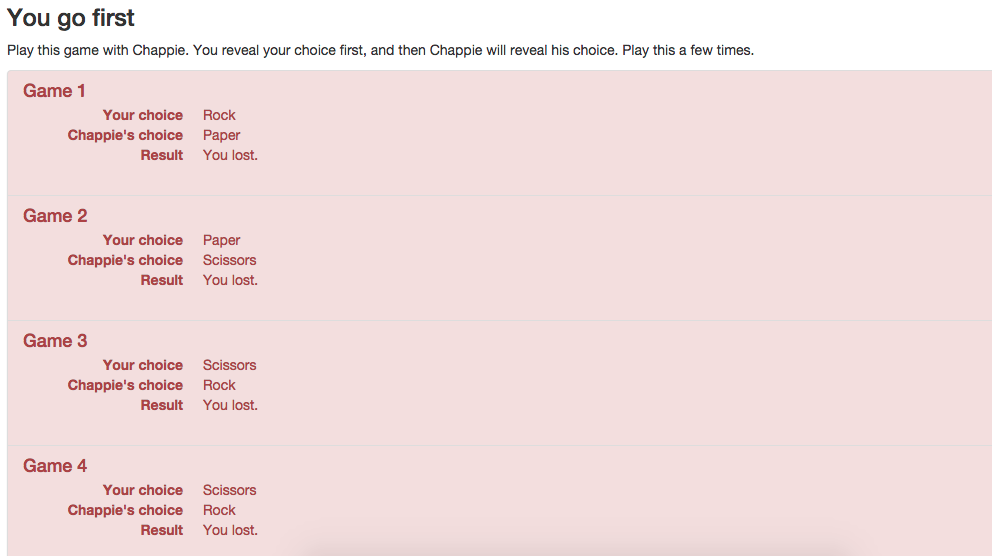
\includegraphics[width=90mm]{image1.png}
			\caption{First Sample \label{overflow}}
		\end{figure}
		\begin{figure}[ht!]
			\centering
			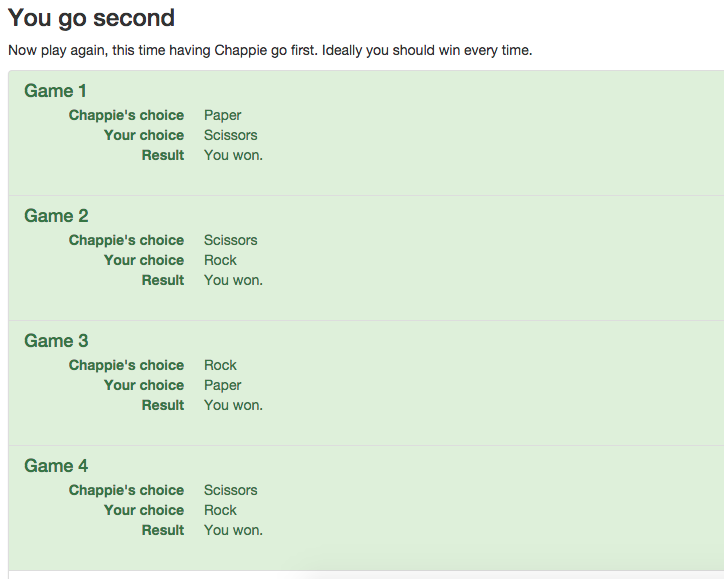
\includegraphics[width=90mm]{image2.png}
			\caption{Second Sample \label{overflow}}
		\end{figure}
		\begin{figure}[ht!]
			\centering
			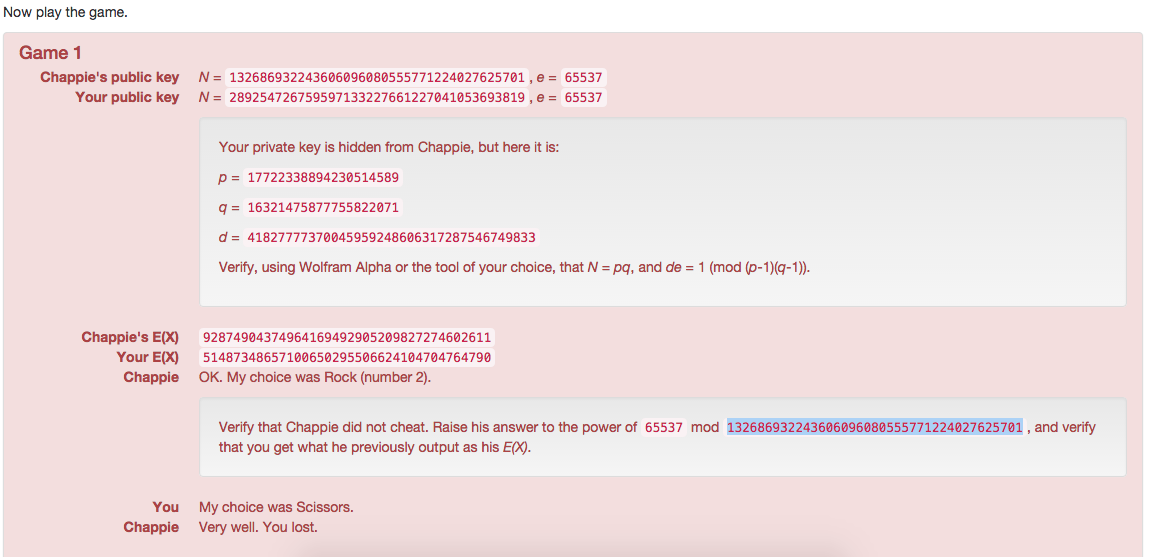
\includegraphics[width=90mm]{image3.png}
			\caption{Third Sample \label{overflow}}
		\end{figure}
		\begin{figure}[ht!]
			\centering
			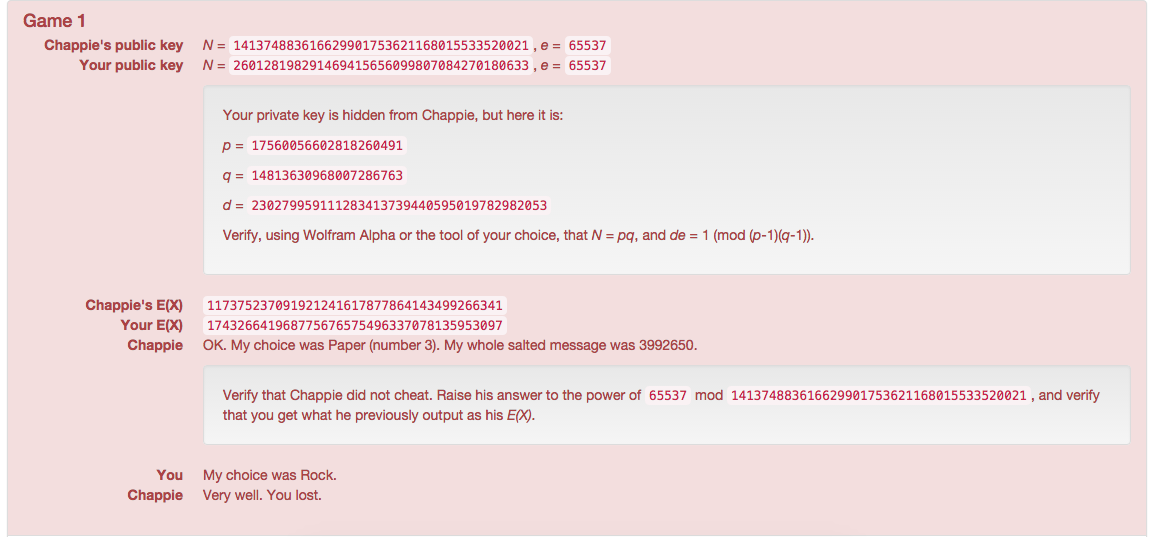
\includegraphics[width=90mm]{image4.png}
			\caption{Fourth Sample \label{overflow}}
		\end{figure}
    
    \item[(b)]
    Personally, I think if only one person encripts it, would be good enough. As in let the first person have the encription and then the second person can just outright say what he chose. Then using the encription from the first person, we can figure out whether or not he is lying. 
    
  \end{enumerate}

\end{enumerate}

\end{document}